% This LaTeX was auto-generated from MATLAB code.
% To make changes, update the MATLAB code and export to LaTeX again.

\documentclass{article}
\usepackage[english, russian]{babel}
\usepackage[utf8]{inputenc}
\usepackage[T1]{fontenc}
\usepackage{lmodern}
\usepackage{graphicx}
\usepackage{color}
\usepackage{listings}
\usepackage{hyperref}
\usepackage{amsmath}
\usepackage{amsfonts}
\usepackage{epstopdf}
\usepackage{matlab}

\sloppy
\epstopdfsetup{outdir=./}
\graphicspath{ {./sound_ca_images/} }

\begin{document}

\begin{par}
\begin{flushleft}
1 Фильтрация сигнала методом скользящего среднего
\end{flushleft}
\end{par}

\begin{par}
\begin{flushleft}
1.1 Инициализация и формирование значений основных параметров
\end{flushleft}
\end{par}

\begin{matlabcode}
clear all; % Очистка памяти
close all; % Закрытие всех окон с графиками
clc; % Очистка окна команд и сообщений
fontSize = 10; % Размер шрифта графиков
tColor = 'b'; % Цвет графиков во временной области
fColor = [1 0.4 0]; % Цвет графиков в частотной области
rColor = [0.2 0.7 0.3]; % Цвет графиков отфильтрованного сигнала
volume = 0.15; % Амплитуда исходного сигнала
f0 = 440; % Частота сигнала, Гц
fd = 16000; % Частота дискретизации, Гц
mean = 0; % Математическое ожидание шума
std = 0.3; % Стандартное отклонение
nK = 100; % Количество накоплений
nT = 20; % Количество периодов отфильтрованного сигнала
dt0 = nT/f0; % Длительность отфильтрованного сигнала, с
N0 = nT*round(fd/f0); % Количество отсчетов отфильтрованного сигнала
dt = nK*dt0; % Длительность зашумлённого сигнала, с
N = N0*nK; % Общее количество отсчетов сигнала
gT = 3; % Количество периодов для визуализации
\end{matlabcode}


\begin{par}
\begin{flushleft}
1.2 Моделирование тонального сигнала
\end{flushleft}
\end{par}

\begin{matlabcode}
t = linspace(0,dt,N); % Формирование области определения во временной области
data = volume*cos(2*pi*f0*t); % Формирование тонального сигнала
% Запись звукового файла с исходным сигналом
audiowrite('sound.wav', data, fd);
figure; plot(t(1:gT*round(fd/f0)), data(1:gT*round(fd/f0)), 'Color', tColor);
set(get(gcf, 'CurrentAxes'), 'FontSize', fontSize); % Изменение шрифта
title('\rm Исходный сигнал во временной области'); % Заголовок
xlabel('Время,\it nT_д\rm, с'); % Надпись оси абсцисс
ylabel('Сигнал,\it x(nT_д )\rm, В'); % Надпись оси ординат
\end{matlabcode}
\begin{center}
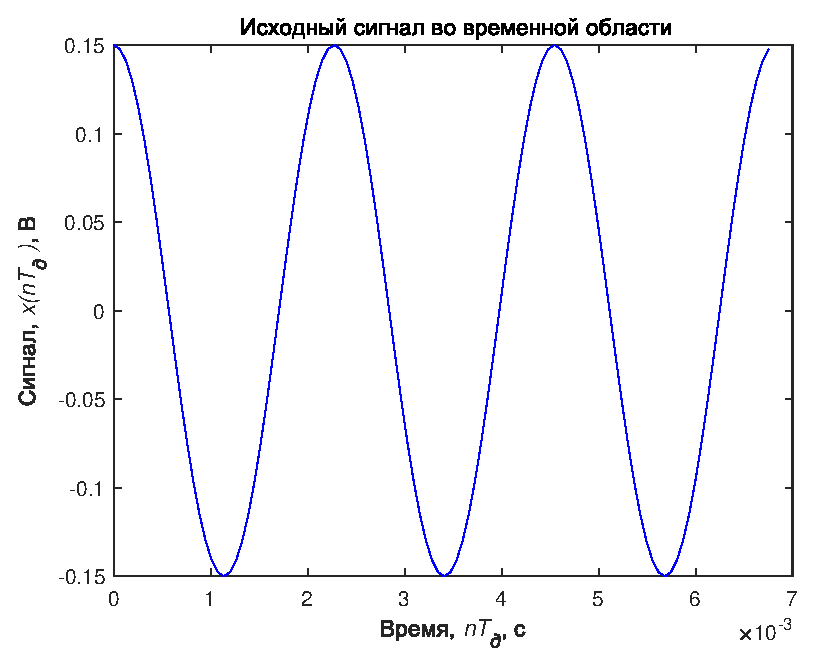
\includegraphics[width=\maxwidth{56.196688409433015em}]{figure_0}
\end{center}


\begin{par}
\begin{flushleft}
1.3 Построение амплитудного спектра тонального сигнала
\end{flushleft}
\end{par}

\begin{matlabcode}
f = linspace(0, fd, N0); % Формирование области определения в частотной области
% Массив отсчётов спектра исходного сигнала
fdata = abs(fft(data(1:N0))/N0);
figure; plot([-fliplr(f(1:end/2)) f(1:end/2)], fftshift(fdata),...
    'Color', fColor, 'LineWidth', 3);
axis([-fd/2 fd/2 0 volume*0.6]); % Диапазон значений осей
set(get(gcf, 'CurrentAxes'), 'FontSize', fontSize); % Изменение шрифта
title('\rm Исходный сигнал в частотной области'); % Заголовок
xlabel('Частота,\it f\rm, Гц'); % Надпись оси абсцисс
ylabel('Амплитуда,\it A(f)\rm, В'); % Надпись оси ординат
\end{matlabcode}
\begin{center}
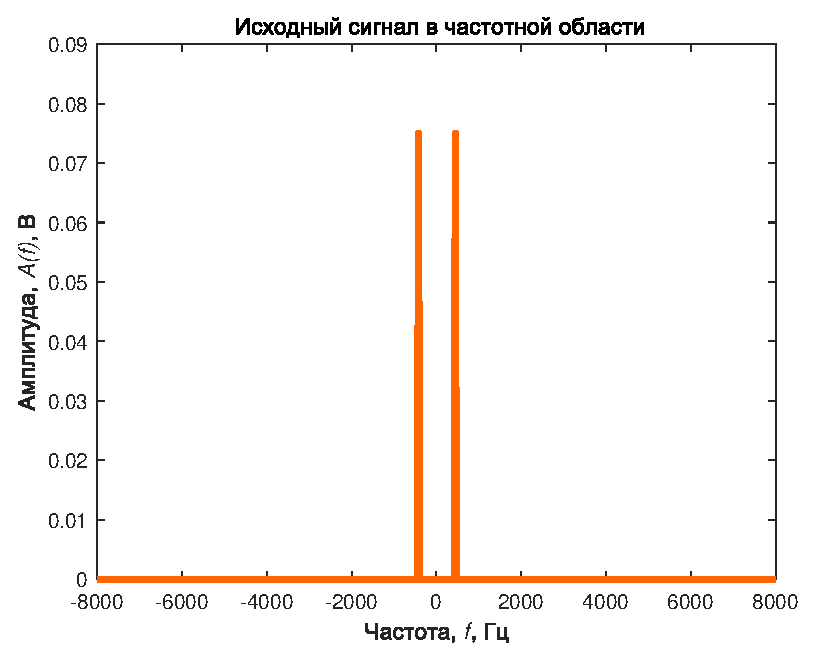
\includegraphics[width=\maxwidth{56.196688409433015em}]{figure_1}
\end{center}


\begin{par}
\begin{flushleft}
1.4 Формирование зашумлённого сигнала
\end{flushleft}
\end{par}

\begin{matlabcode}
ny = normrnd(mean, std, [1,N]); % Массив отсчётов шума по норм. распределению
ndata = data + ny; % Добавление шума к исходному сигналу
% Запись звукового файла с зашумлённым сигналом
mdata = reshape(ndata, [N0,nK]).'; % Разделение сигнала на nK накоплений
figure; plot(t(1:gT*round(fd/f0)), mdata(1,1:gT*round(fd/f0)), 'Color', tColor);
set(get(gcf, 'CurrentAxes'), 'FontSize', fontSize); % Изменение шрифта
title('\rm Зашумлённый сигнал во временной области'); % Заголовок
xlabel('Время,\it nT_д\rm, с'); % Надпись оси абсцисс
ylabel('Сигнал,\it x(nT_д )\rm, В'); % Надпись оси ординат
\end{matlabcode}
\begin{center}
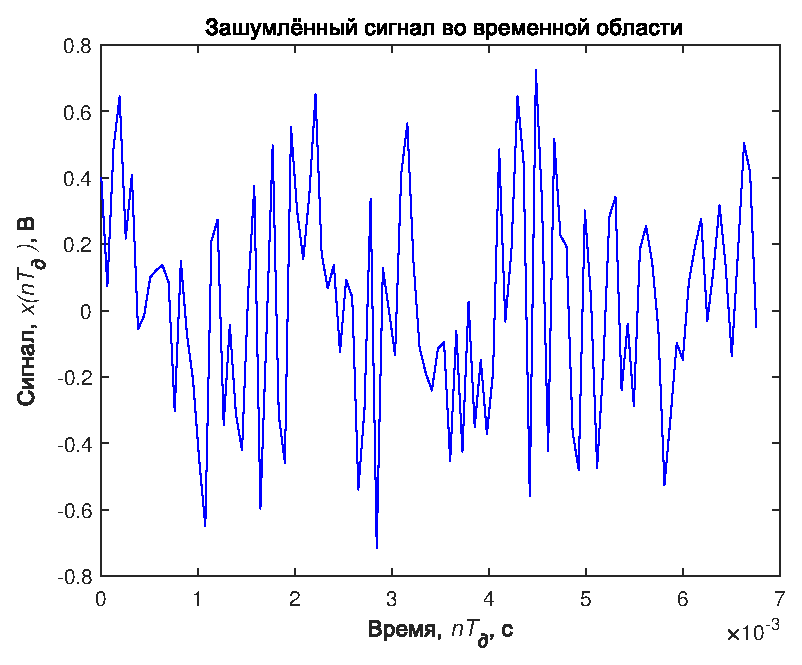
\includegraphics[width=\maxwidth{56.196688409433015em}]{figure_2}
\end{center}


\begin{par}
\begin{flushleft}
1.5 Построение амплитудного спектра зашумлённого сигнала
\end{flushleft}
\end{par}

\begin{matlabcode}
% Массив отсчётов спектра зашумлённого сигнала
fmdata = abs(fft(mdata(1,:))/N0);
figure; plot([-fliplr(f(1:end/2)) f(1:end/2)], fftshift(fmdata),...
    'Color', fColor, 'LineWidth', 3);
axis([-fd/2 fd/2 0 volume*0.6]); % Диапазон значений осей
set(get(gcf, 'CurrentAxes'), 'FontSize', fontSize); % Изменение шрифта
title('\rm Зашумлённый сигнал в частотной области'); % Заголовок
xlabel('Частота,\it f\rm, Гц'); % Надпись оси абсцисс
ylabel('Амплитуда,\it A(f)\rm, В'); % Надпись оси ординат
\end{matlabcode}
\begin{center}
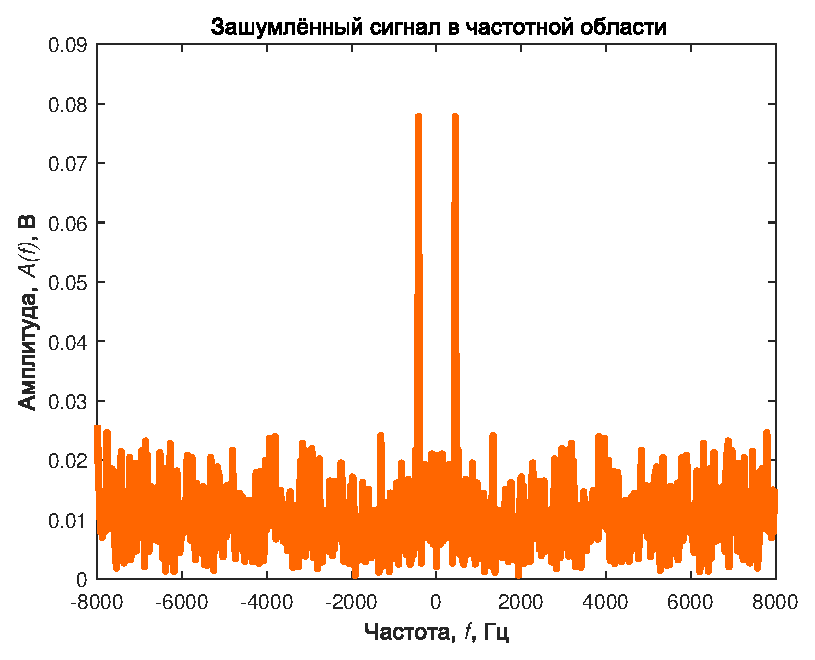
\includegraphics[width=\maxwidth{56.196688409433015em}]{figure_3}
\end{center}


\begin{par}
\begin{flushleft}
1.6 Фильтрация методом когерентного накопления
\end{flushleft}
\end{par}

\begin{matlabcode}
% Фильтрация методом когерентного накопления с количеством накоплений nK
sdata = sum(mdata)./nK;
% Запись звукового файла с отфильтрованным сигналом
audiowrite('filter.wav', sdata, fd);
% Построение графика с зашумлённым и отфильтрованным сигналами
figure; plot(t(1:gT*round(fd/f0)), mdata(1,1:gT*round(fd/f0)), 'Color', tColor); hold on;
plot(t(1:gT*round(fd/f0)), sdata(1:gT*round(fd/f0)), 'Color', rColor, 'LineWidth', 2);
set(get(gcf, 'CurrentAxes'), 'FontSize', fontSize); % Изменение шрифта
title('\rm Отфильтрованный сигнал во временной области'); % Заголовок
xlabel('Время,\it nT_д\rm, с'); % Надпись оси абсцисс
ylabel('Сигнал,\it x(nT_д )\rm, В'); % Надпись оси ординат
\end{matlabcode}
\begin{center}
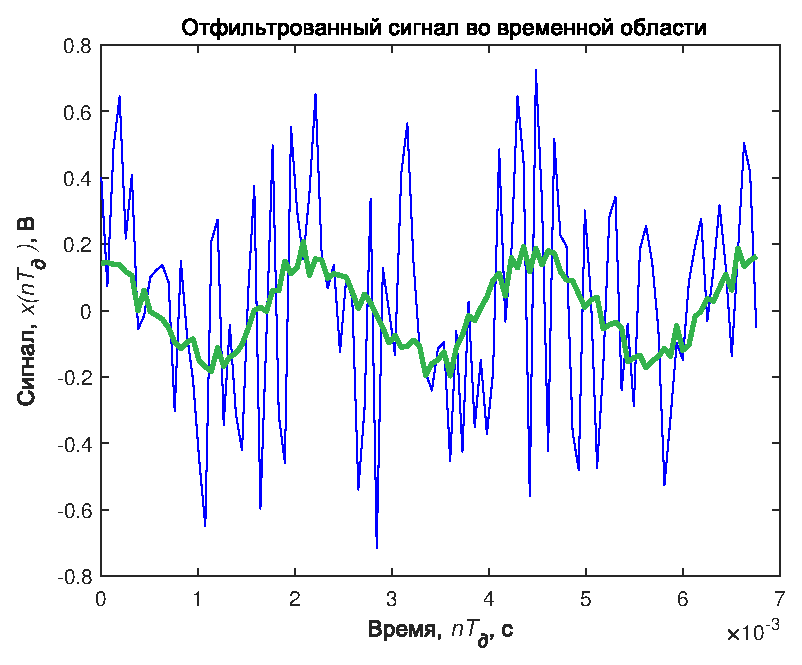
\includegraphics[width=\maxwidth{56.196688409433015em}]{figure_4}
\end{center}


\begin{par}
\begin{flushleft}
1.7 Построение амплитудных спектров зашумлённого и отфильтрованного сигналов
\end{flushleft}
\end{par}

\begin{matlabcode}
% Массив отсчётов спектра отфильтрованного сигнала
fsdata = abs(fft(sdata)/N0); % Формирование значений
figure; plot([-fliplr(f(1:end/2)) f(1:end/2)], fftshift(fmdata),...
    'Color', fColor, 'LineWidth', 3); hold on;
plot([-fliplr(f(1:end/2)) f(1:end/2)], fftshift(fsdata),...
    'Color', rColor, 'LineWidth', 2);
axis([-fd/2 fd/2 0 volume*0.6]); % Диапазон значений осей
set(get(gcf, 'CurrentAxes'), 'FontSize', fontSize); % Изменение шрифта
title('\rm Отфильтрованный сигнал в частотной области'); % Заголовок
xlabel('Частота,\it f\rm, Гц'); % Надпись оси абсцисс
ylabel('Амплитуда,\it A(f)\rm, В'); % Надпись оси ординат
\end{matlabcode}
\begin{center}
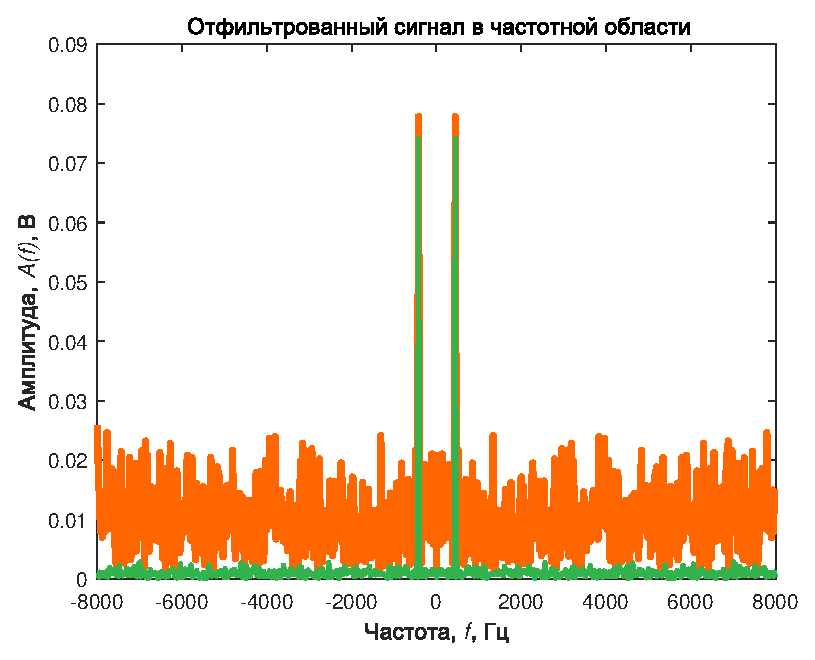
\includegraphics[width=\maxwidth{56.196688409433015em}]{figure_5}
\end{center}

\end{document}
